\documentclass[11pt,a4paper]{article}

\usepackage[utf8]{inputenc}
\usepackage[T1]{fontenc}
\usepackage[brazil]{babel}
\usepackage[top=2.2cm, bottom=2.2cm, left=2.2cm, right=2.2cm]{geometry}
\usepackage{enumitem}
\usepackage{parskip}
\usepackage{microtype}
\usepackage{graphicx}

\begin{document}

\begin{center}
  {\large\textbf{Mini-avaliação --- Ciclo Hamiltoniano}}\\
  %{\textbullet{} 10 min \textbullet{} 10 pontos}
\end{center}

\hrule
\vspace{6pt}

% ============================================================
\section*{Questão 1 \hfill (3 pontos)}

Marque a alternativa \textbf{correta} sobre o problema do Ciclo Hamiltoniano.

\begin{enumerate}[label=(\alph*),leftmargin=*]
  \item Consiste em percorrer todas as \textbf{arestas} de um grafo exatamente uma vez.
  \item Consiste em visitar todos os \textbf{vértices} de um grafo exatamente uma vez, retornando ao vértice inicial.
  \item Consiste em encontrar o caminho mais curto entre dois vértices de um grafo.
  \item Consiste em colorir os vértices de um grafo com o menor número possível de cores.
\end{enumerate}

\textit{Resposta correta: (b).}

% ============================================================
\section*{Questão 2 \hfill (3 pontos)}

Sobre o Ciclo Hamiltoniano, marque \textbf{V} (verdadeiro) ou \textbf{F} (falso):

\begin{enumerate}[label=(\alph*),leftmargin=*,itemsep=4pt]
  \item (\hspace{1em}) Verificar se uma sequência candidata de vértices é um ciclo hamiltoniano pode ser feito de forma rápida.
  \item (\hspace{1em}) Encontrar um ciclo hamiltoniano em um grafo qualquer é, no caso geral, um problema computacionalmente difícil.
  \item (\hspace{1em}) Como o problema é NP-completo, ele é impossível de ser resolvido em qualquer situação.
\end{enumerate}

\textit{Respostas: (a) V, (b) V, (c) F. \quad 1 ponto por item.}

% ============================================================
\section*{Questão 3 \hfill (4 pontos)}

Considere o grafo abaixo, com vértices $\{A, B, C, D\}$ e arestas
$\{AB,\ BC,\ CD,\ DA,\ AC\}$.

\begin{center}
  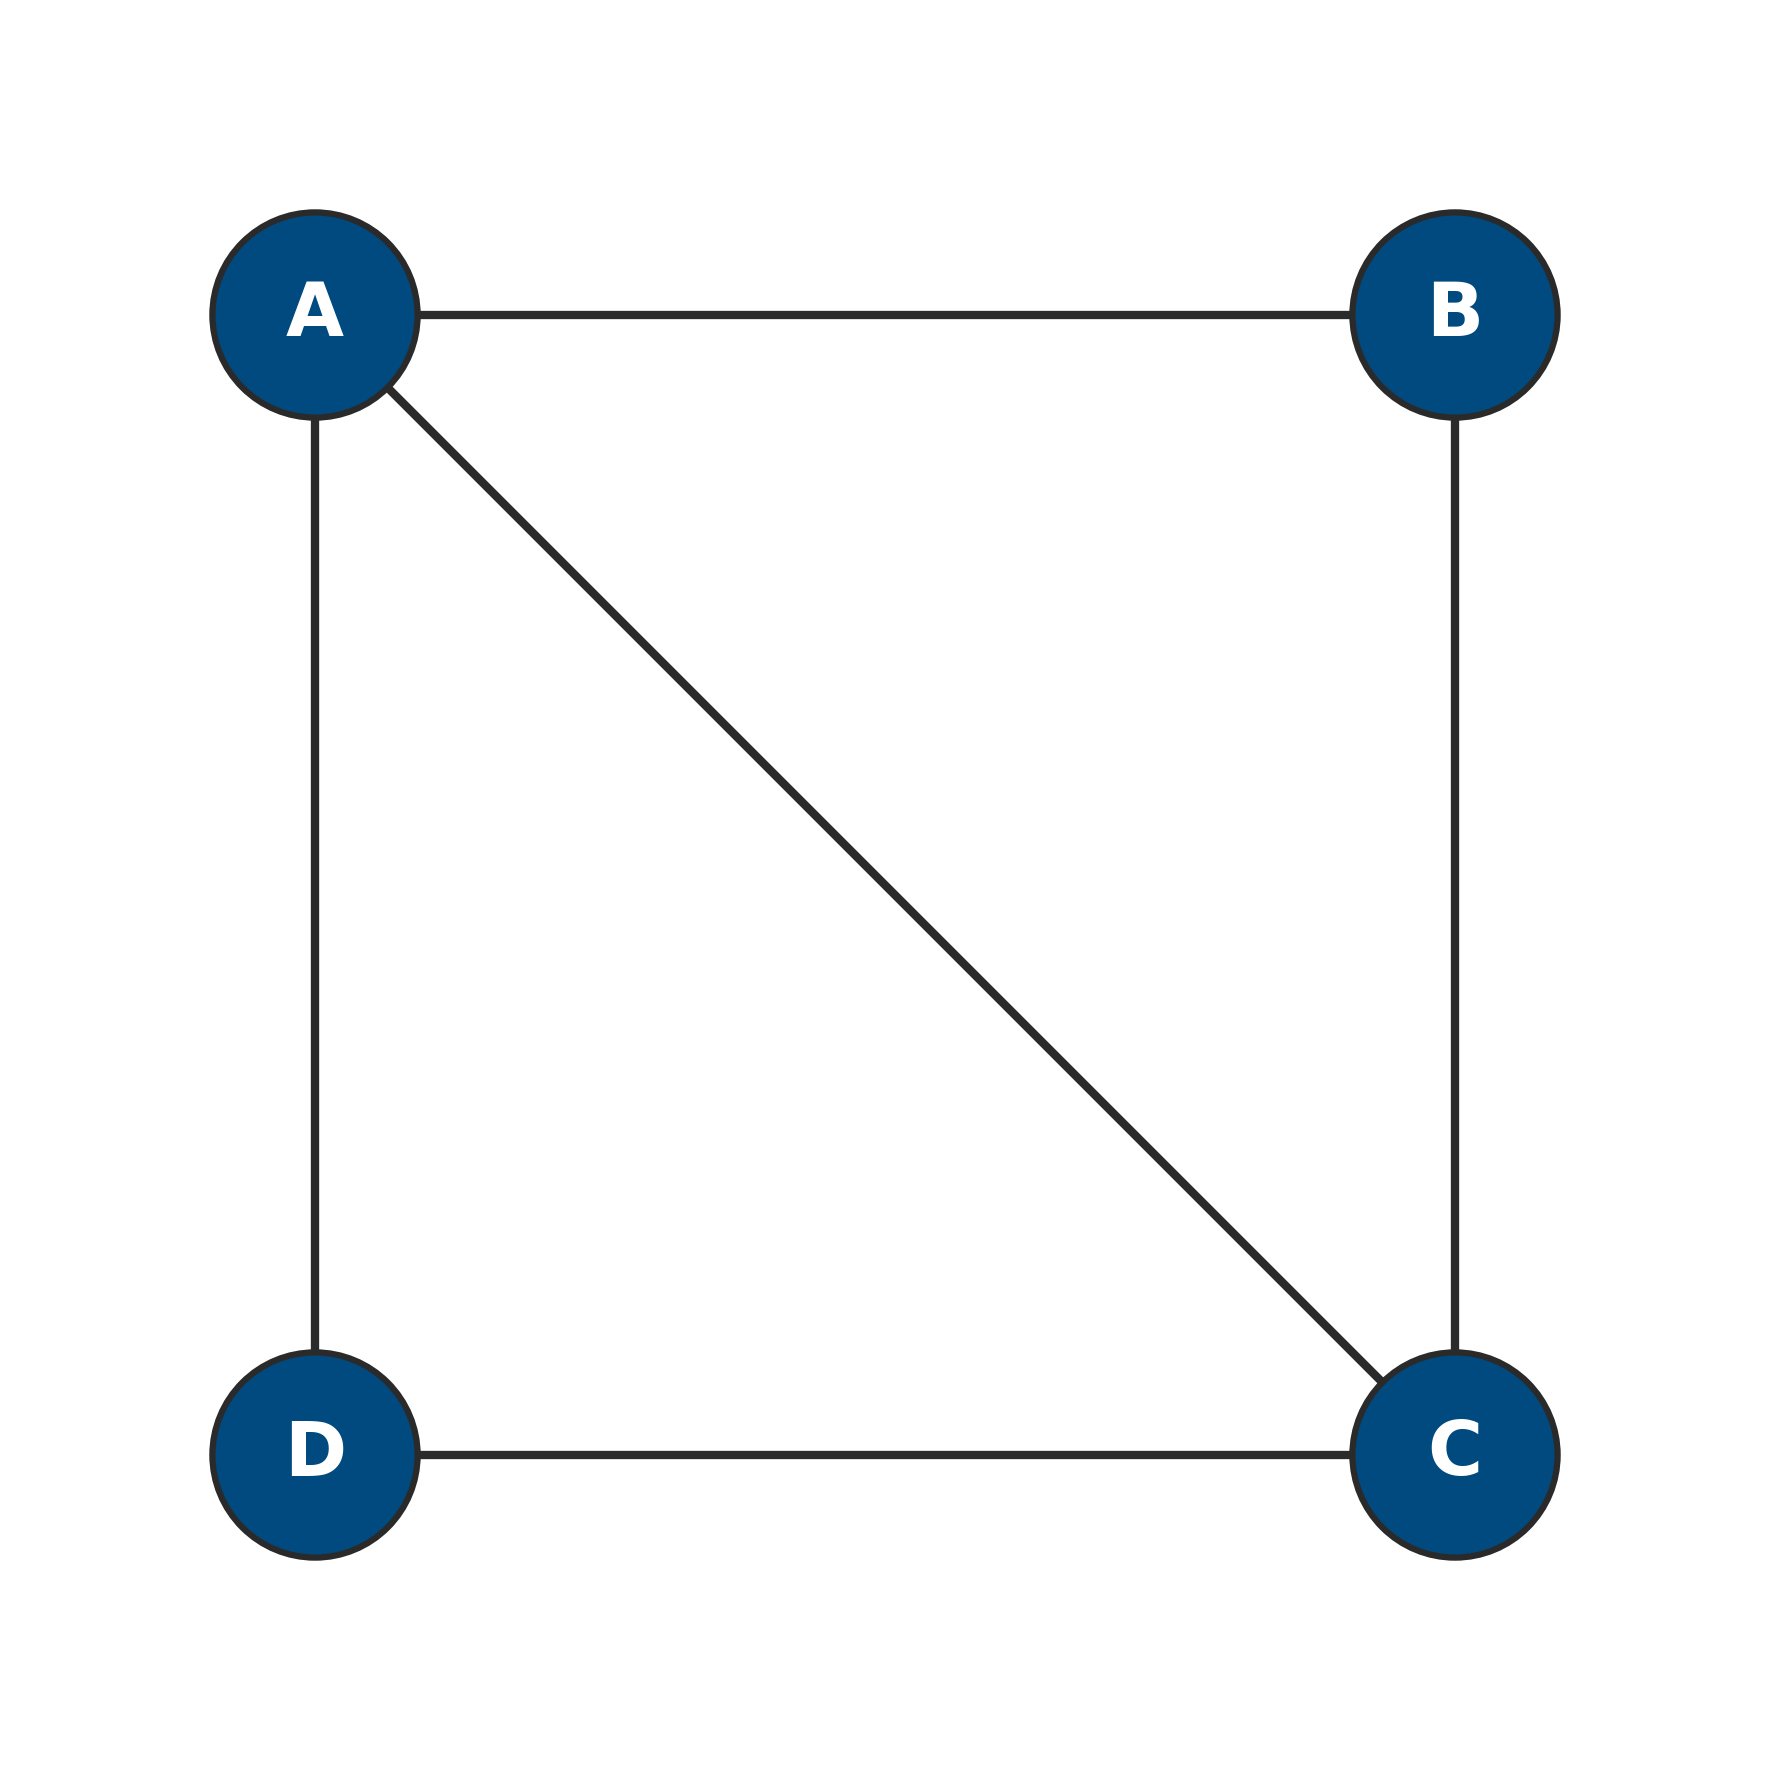
\includegraphics[width=0.35\linewidth]{grafo_q3.png}
\end{center}

\textbf{(a)} A sequência $A \to B \to C \to D \to A$ é um ciclo hamiltoniano? Justifique brevemente. \hfill (2 pontos)

\vspace{30pt}

\textbf{(b)} Qual é a diferença principal entre um Ciclo \textbf{Euleriano} e um Ciclo \textbf{Hamiltoniano}? Responda em uma frase. \hfill (2 pontos)

\vspace{30pt}

\textit{Respostas esperadas:}

\textit{(a) \textbf{Sim.} Todos os vértices ($A, B, C, D$) aparecem exatamente uma vez, todas as arestas consecutivas existem no grafo ($AB, BC, CD, DA$), e o ciclo retorna ao vértice inicial.}

\textit{(b) O Ciclo Euleriano percorre todas as \textbf{arestas} do grafo exatamente uma vez; o Ciclo Hamiltoniano visita todos os \textbf{vértices} do grafo exatamente uma vez.}

\end{document}